\documentclass{standalone}
\usepackage{tikz}
\usepackage{nono}
\begin{document}
  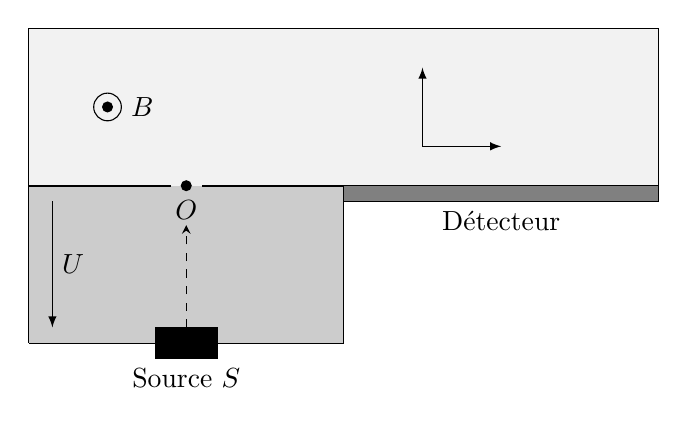
\begin{tikzpicture}
    \fill[gray!40](0,0) rectangle ++(4,2);
    \fill[gray!10](0,2) rectangle ++(8,2);
    \draw (0,0) -- ++(0,4) -- ++(8,0) -- ++(0,-2) -- ++(-4,0) -- ++(0,-2) --++(-4, 0);
    \draw[thick] (0, 2) -- ++(1.8,0) ++(0.4,0) --++(1.8,0);
    \fill[black] (2, 2) circle(2pt) node[below, yshift=-2pt]{$O$ };
    \draw[-latex] (0.3, 1.8) -- (0.3, 0.2) node[right , midway] {$U$};
    \draw[dashed, -stealth] (2,0.2) -- (2, 1.5) ;
    \draw[fill=gray] (4, 1.8) rectangle (8, 2);
    \draw (6, 1.8) node[below]{Détecteur};
    \fill[black] (1.6, -0.2) rectangle (2.4, 0.2);
    \draw (2,-0.2) node[below]{Source $S$};
    \draw (1, 3) circle(5pt) node[right, xshift=5pt] {$\vv{B}$}; 
    \fill (1,3) circle(2pt);
    \draw[-latex] (5, 2.5) -- ++(1,0) node[right] {$\vex $};  
    \draw[-latex] (5, 2.5) -- ++(0,1) node[right] {$\vey $};  
  \end{tikzpicture}
\end{document}
